\ifx\wholebook\relax \else

\documentclass[b5paper]{ctexart}
\usepackage[nomarginpar
  %, margin=.5in
]{geometry}

\addtolength{\oddsidemargin}{-0.05in}
\addtolength{\evensidemargin}{-0.05in}
\addtolength{\textwidth}{0.1in}

\usepackage[cn]{../prelude}

\setcounter{page}{1}

\begin{document}

\title{分数}

\author{刘新宇
\thanks{{\bfseries 刘新宇} \newline
  Email: liuxinyu99@hotmail.com \newline}
  }

\maketitle
\fi

\markboth{分数}{数的旅程}

\ifx\wholebook\relax
\chapter{分数}
\fi

\epigraph{此曲只应天上有,人间能得几回闻。}{杜甫《赠花卿》}

2015年9月14日,美国LIGO\footnote{激光干涉引力波}天文台探测到一个神秘信号GW150914。它来自13亿光年之外的一次惊天动地的奇观:一对双黑洞天体彼此靠近、吸引,旋转着合并到一起(如\cref{fig:gravitational-wave})。它们巨大引力激起的“涟漪”穿越13亿年时空\footnote{根据爱因斯坦的广义相对论,引力波以光速传播。}到达了地球。物理学家们花了几个月的事件进行数据分析,排除了可能的干扰因素,最终于2016年2月11日正式宣布:这是人类首次探测到了引力波,证实了爱因斯坦在百年前通过广义相对论做出的预言。LIGO的物理学家们把引力波转换成声音信号,我们得以首次听到来自宇宙深处的“天籁之音”。

\begin{figure}[htbp]
 \centering
 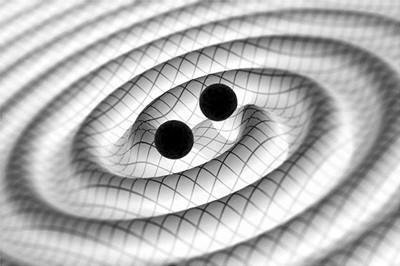
\includegraphics[scale=0.35]{img/gravitational-wave}
 \caption{双黑洞彼此合并过程中产生的引力波示意。}
 \label{fig:gravitational-wave}
\end{figure}

2500年前,正是追寻天籁之音的过程,使得古希腊的先贤毕达哥拉斯发现了音乐背后的数学秘密。相传有一天毕达哥拉斯经过铁匠铺,听到从里面传出了悦耳的声音。这些声音是铁匠们用不同重量的铁锤一起敲打铁砧时产生的。巴洛克时期的音乐家亨德尔有一部作品叫做《快乐的铁匠》(作品编号:HWV430)。毕达哥拉斯注意到有些声音是和谐的,而另一些不和谐。他进一步发现当铁锤的重量比恰好是12、9、8、6时,敲打的声音是和谐的。毕达哥拉斯敏锐地发现了音乐背后的数字规律:

\begin{itemize}
\item 比例$12:6$(即$2:1$)对应纯8度音;
\item 比例$9:6$(即$3:2$)对应纯5度音;
\item 比例$12:9$(即$4:3$)对应纯4度音;
\item 比例$9:8$对应纯2度音。
\end{itemize}

%% \begin{figure}[htbp]
%%  \centering
%%  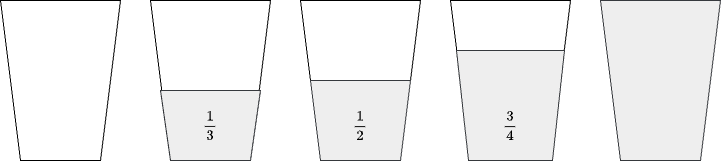
\includegraphics[scale=0.4]{img/cups}
%%  \caption{盛有不同水的杯子}
%%  \label{fig:fraction-cups}
%% \end{figure}

这个故事非常流行,如\ref{fig:pythagoras-music}所示。这幅四联木刻连环画展示了毕达哥拉斯先是聆听到铁匠们挥舞铁锤敲打,然后他开始进行\underdot{定量}研究,包括敲打不同重量的钟,敲打盛有不同水的杯子,弹拨坠有不同重量的琴弦,吹奏不同长度的笛子。但这个故事禁不起推敲,第二幅图和第一幅图是相互矛盾的。我们可以自己动手验证一下。依照第二幅图中的样子,用几个同样的杯子盛上不同的水,然后用不同大小的勺子敲击。我们会发现音调的高低是由杯子而不是勺子决定的。同理,铁匠铺传出的音调高低是由铁砧而不是锤子决定的。但第一幅图中只有一个铁砧。这组连环画还有别的问题。铁锤、钟、杯子、琴弦上的砝码、笛子上的数字4、6、8、9、12、16是印度——阿拉伯数字(见第\ref{sec:hindu-arabic-numerals}节),要到十三、十四世纪才传入欧洲。古希腊的毕达哥拉斯不可能用这样的数字。尽管如此,这组连环画仍然反映了毕达哥拉斯求知好学,善于思考,动手实践进行定量研究的治学传统。

\begin{figure}[htbp]
 \centering
 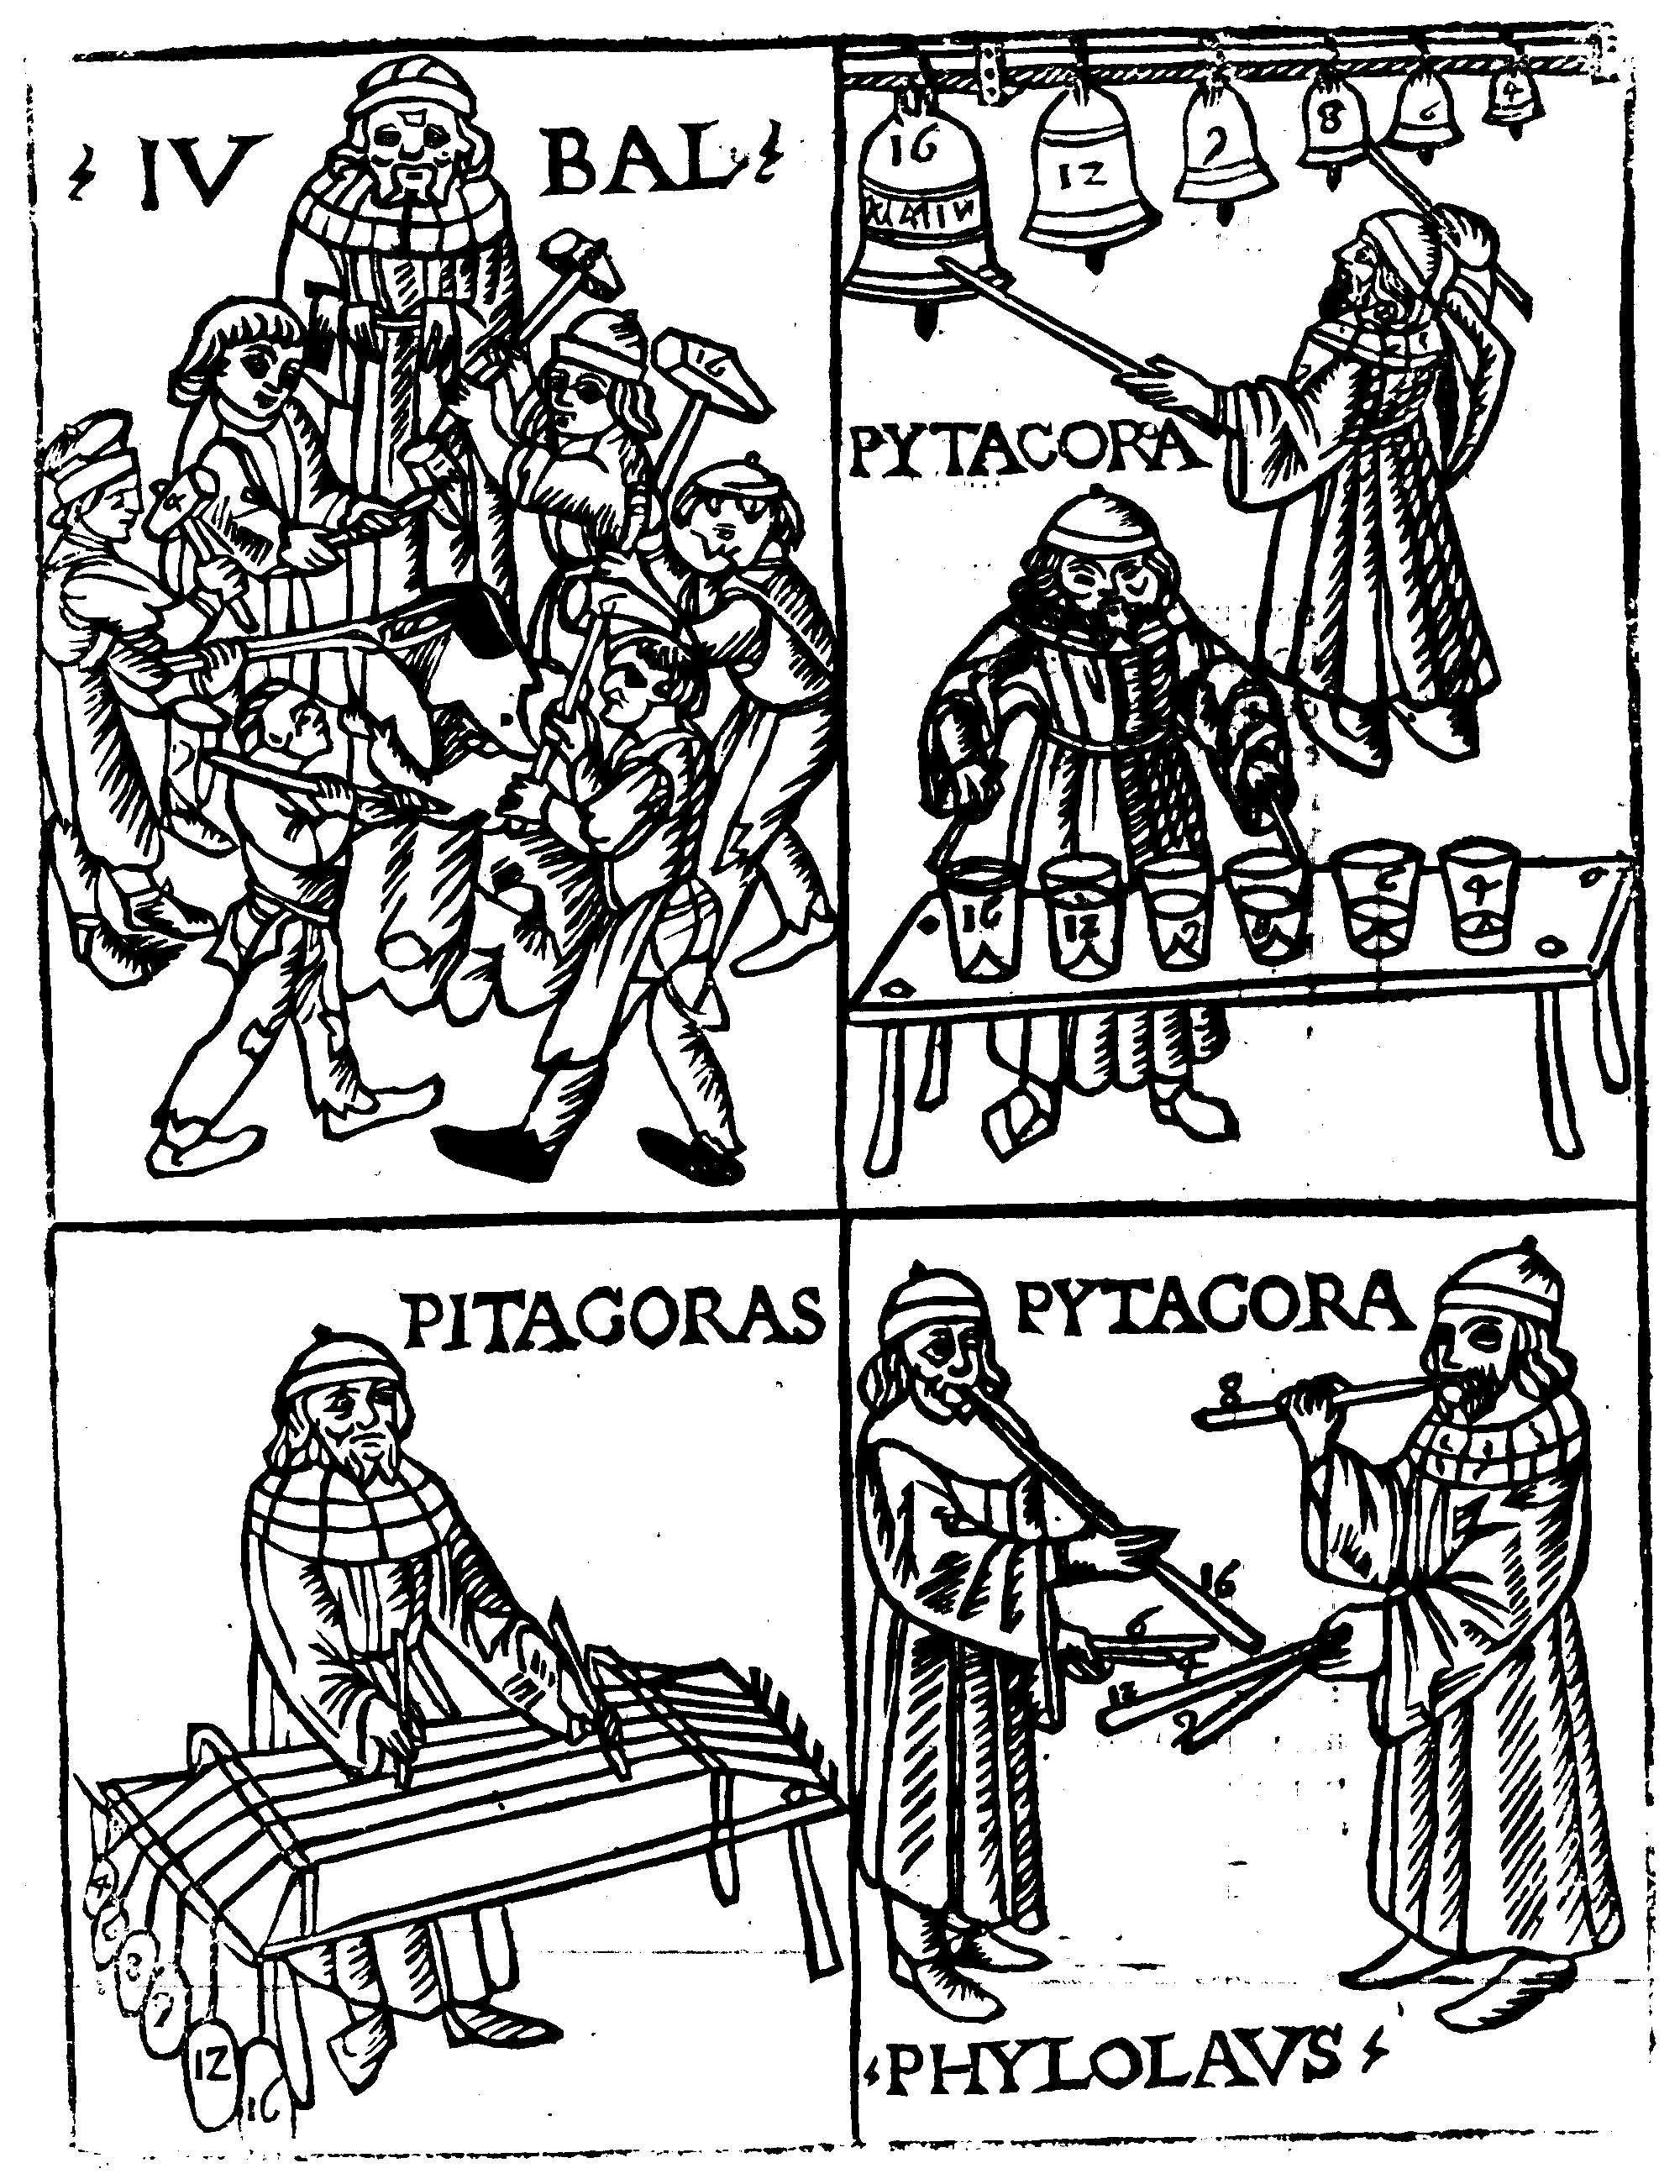
\includegraphics[scale=0.1]{img/pythagoras-music}
 \caption{毕达哥拉斯与音乐,出自1492年(或1480年)弗兰奇诺・加富里奥《乐理》中的木刻插页。}
 %% Woodcut showing Pythagoras with bells, a kind of glass harmonica, a monochord and (organ?) pipes in Pythagorean tuning. From Theorica musicae by Franchino Gaffurio, 1492 (1480?)
 %% https://commons.wikimedia.org/wiki/File:Gaffurio_Pythagoras.png
 \label{fig:pythagoras-music}
\end{figure}

古希腊的乐器叫做里尔琴(Lyre,也译作里拉琴、莱雅琴、诗琴),是一种七弦琴(见\cref{fig:lyre}),在很多场合已经成为代表音乐的符号。我们推测毕达哥拉斯把琴弦的一半,也就是$\frac{1}{2}$张紧弹奏,获得了8度音;把琴弦的$\frac{2}{3}$张紧弹奏,获得了5度音;把琴弦的$\frac{3}{4}$张紧弹奏,获得了4度音;这些音调之间的关系如\cref{fig:octave}所示。

\begin{figure}[htbp]
 \centering
 \subcaptionbox{绘有太阳神阿波罗手持里尔琴的盘子,约公元前480~470年,藏于雅典德尔菲博物馆。}{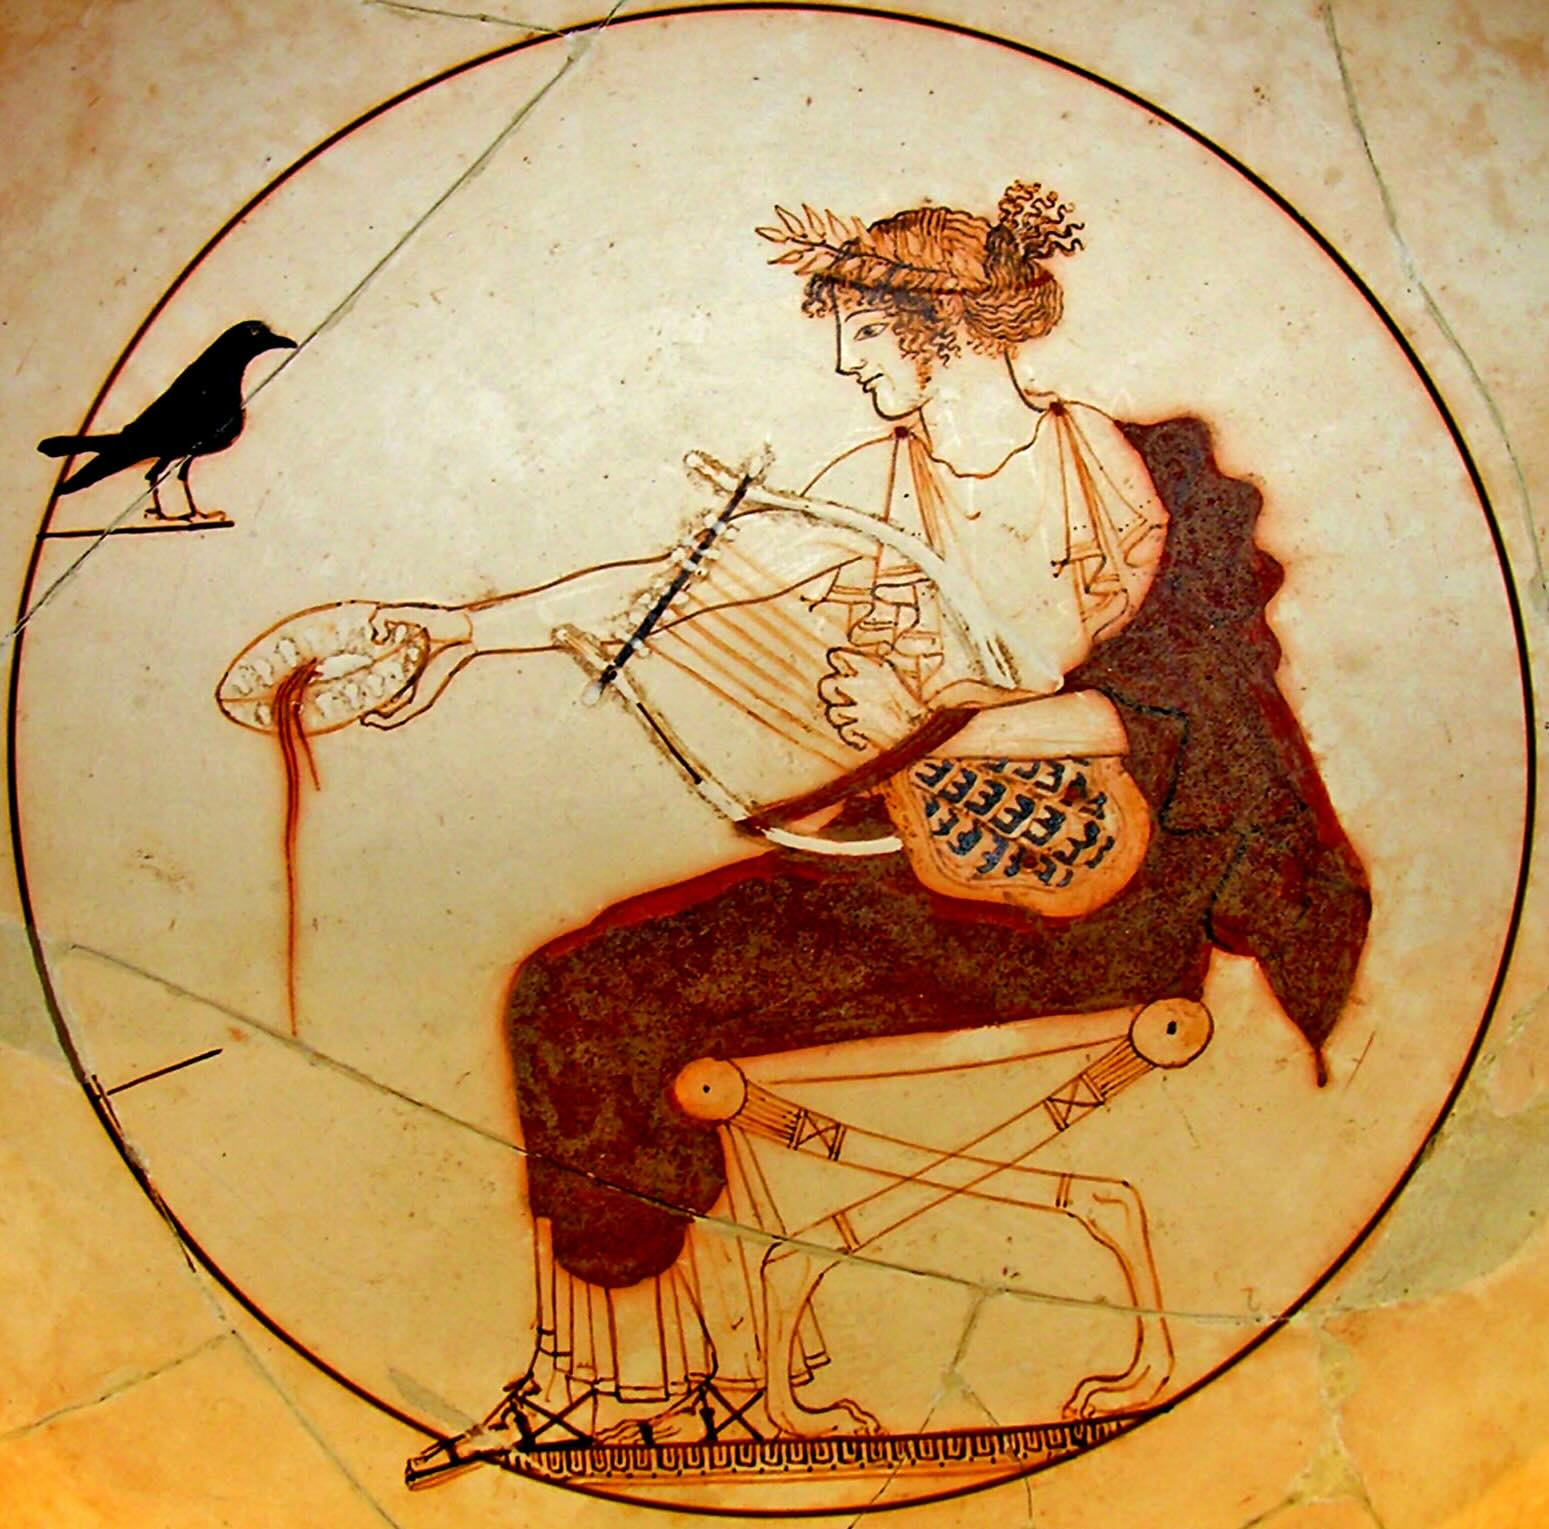
\includegraphics[scale=0.4]{img/apollo-with-lyre}}
 \subcaptionbox{里尔琴符号}{
\includegraphics[scale=0.35]{img/lyre-icon}}
 %% https://www.worldhistory.org/image/986/apollo-with-lyre/
 \label{fig:lyre}
\end{figure}

毕达哥拉斯通过数学,具体说是\underdot{分数与比例}奠定了西方音乐的理论基础。他认为整个宇宙是一把巨大的里尔琴,古希腊人所知道的七个天体(日月和五大行星水星、金星、火星、木星、土星)是琴上的七根弦,在不同的音调上震动。而数与比例代表着宇宙和谐的天籁之音。

\begin{figure}[htbp]
 \centering
 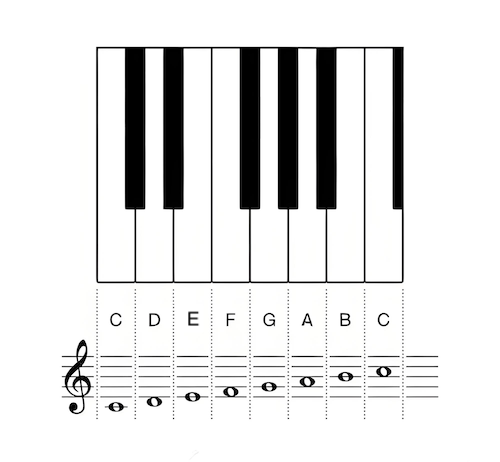
\includegraphics[scale=0.4]{img/octave}
 \caption{两个C间隔8度,琴弦比$2:1$;C与G间隔5度,琴弦比$3:2$;C与F间隔4度,琴弦比$4:3$。}
 \label{fig:octave}
\end{figure}

分数的历史比零和负数还要长。古代中国在春秋时代(公元前770年~前476年)的《左传》中,规定了诸侯的都城大小:最大不可超过周文王国都的三分之一,中等的不可超过五分之一,小的不可超过九分之一。但它们只是表达某种部分的量的词语,而不是真正意义上的分数,因为它们没有直接参与加减乘除运算。古代中国要到汉代才发展出完整的分数计算规则,见\ref{sec:chinese-fractions}节。最早的分数出现在古埃及。

\section{埃及分数}
我们是通过两份重要的古代文件了解到埃及分数的。它们是莱茵德纸草书(见\cref{fig:rhind-papyrus})和莫斯科纸草书(见\cref{fig:moscow-papyrus})。所谓纸草书\footnote{英文Papyrus,是纸的英文paper的字源}是古埃及广泛使用的书写载体。它用当时盛产于尼罗河三角洲的纸莎草的茎制成。经过切片、浸泡、压制、干燥制成。在公元前3000年左右甚至出口到希腊。莎草纸在埃及的干燥气候下可以很好地保存,经历千年而不腐坏。但在潮湿的环境下,很容易霉变损毁。这两份保留了古埃及数学成果的纸草书异常珍贵。它们一份由英国埃及学者莱茵德(Rhind)于1858年购得,现藏于大英博物馆。内容是公元前1650年前后的教科书,作者是书记官阿梅斯\footnote{Ahmes,也译作阿默斯。}。莫斯科纸草书又名戈列尼雪夫纸草书,由俄罗斯贵族戈列尼雪夫于1893年在埃及购得,现藏于莫斯科普希金精细艺术博物馆。作者是约公元前1890年的一位佚名作者。

\begin{figure}[htbp]
 \centering
 \subcaptionbox{莱茵德纸草书局部\label{fig:rhind-papyrus}}{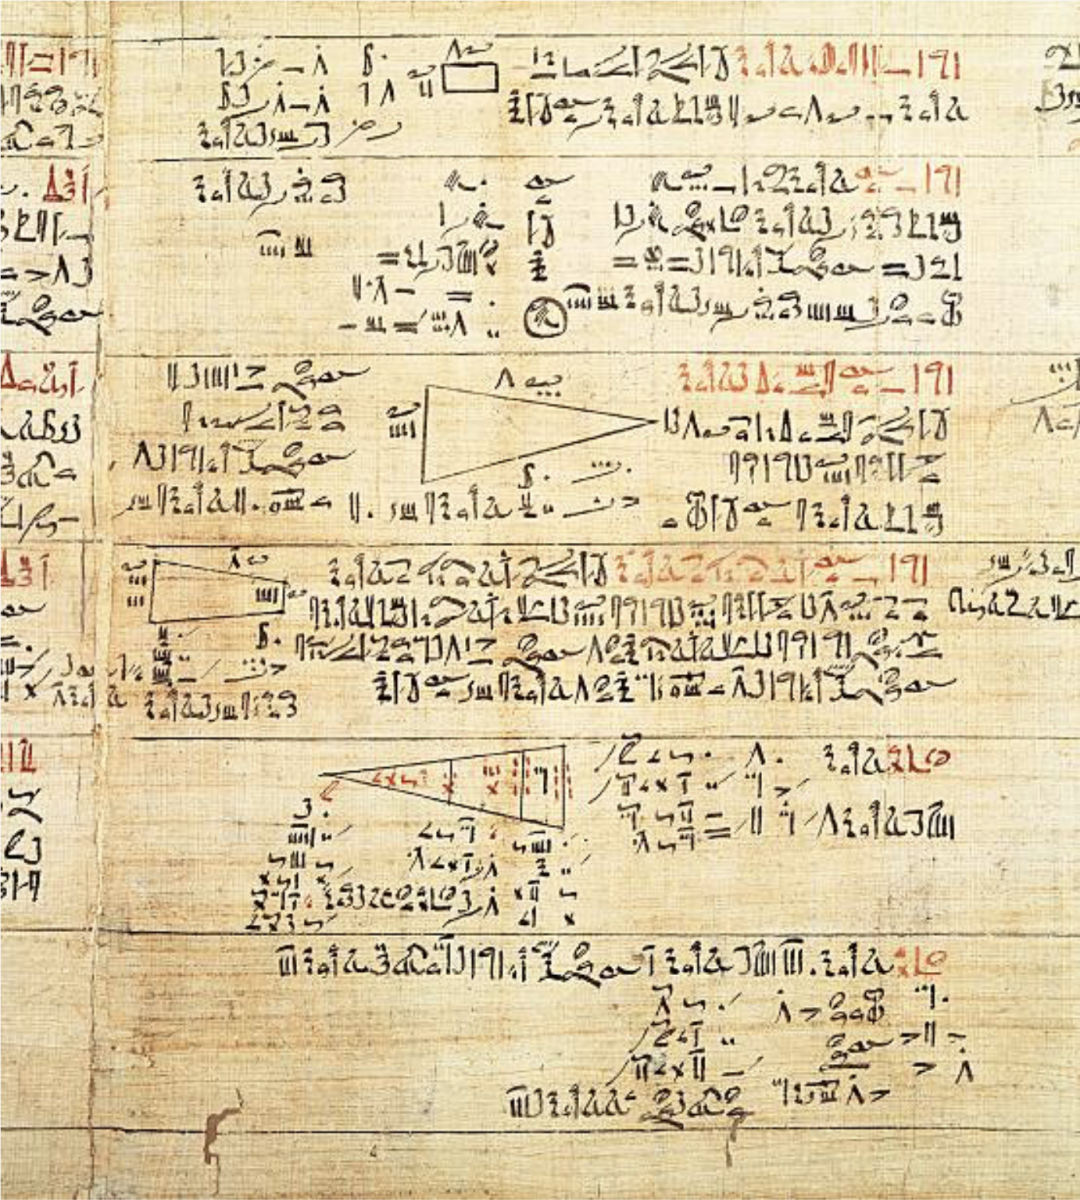
\includegraphics[scale=0.2]{img/rhind-papyrus-part}} \quad
 \subcaptionbox{莫斯科纸草书局部\label{fig:moscow-papyrus}}{ 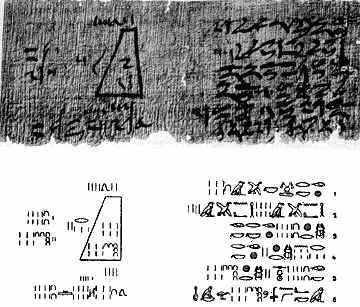
\includegraphics[scale=0.4]{img/moscow-papyrus}}
 %% https://www.britishmuseum.org/collection/image/366139001
 %% https://old.maa.org/press/periodicals/convergence/mathematical-treasure-the-rhind-and-moscow-mathematical-papyri
 %% https://mathshistory.st-andrews.ac.uk/HistTopics/Egyptian_papyri/
\end{figure}

这两份文物反映了古埃及人已使用分数参与运算解决问题。但古埃及的分数有一个既奇怪又合理的特点——所有的分子都是1。因此被称为“单位分数”。在古埃及象形文字(圣书体,见\ref{sec:rosetta-stone}节)中,在数字$a$上方写(画)一个“眼睛”来表示$\frac{1}{a}$,如所\cref{fig:egyptian-fractions}示,表示$\frac{1}{5}$和$\frac{1}{15}$。单位分数的意义是直观易懂的。$\frac{1}{3}$表示把某物均分3份后每份的量,$\frac{1}{5}$是均分5份后每份的量,$\frac{1}{a}$是均分$a$份后每份的量。

\begin{figure}[htbp]
 \centering
 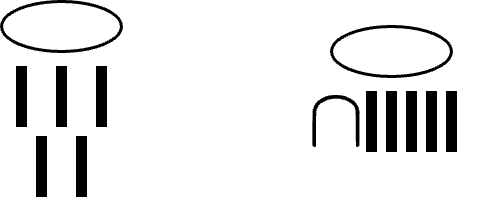
\includegraphics[scale=0.3]{img/egyptian-fractions}
 \caption{埃及分数$\frac{1}{5}$和$\frac{1}{15}$}
 \label{fig:egyptian-fractions}
\end{figure}

但是$\frac{3}{4}$、$\frac{2}{7}$这样的值分子不为1,古埃及人就把它们表示为单位分数之和。例如$\frac{3}{4} = \frac{1}{2} + \frac{1}{4}$,写成象形文字如\cref{fig:sum-egyptian-fractions}左侧所示。中间的符号象征着一个人行走的双腿。如果行走的方向同书写方向一致表示相加,行走的方向同书写的方向相反表示相减。\cref{fig:sum-egyptian-fractions}右侧表示$\frac{2}{5} (= \frac{1}{3} + \frac{1}{15})$。将一个值表示为单位分数的和时,古埃及人要求每个单位分数都不同,不允许重复。因此$\frac{2}{7}$不能写成$\frac{1}{7} + \frac{1}{7}$而要写成$\frac{1}{4} + \frac{1}{28}$。某些情况下,仅仅分解为两个单位分数是不够的。例如莱茵德纸草书上将$\frac{2}{29}$分解为$\frac{2}{29} = \frac{1}{24} + \frac{1}{58} + \frac{1}{174} + \frac{1}{232}$。并且分解方式是不唯一的,例如$\frac{2}{29} = \frac{1}{15} + \frac{1}{435} = \frac{1}{16} + \frac{1}{232} + \frac{1}{464}$。这样的分解没有明显的规律,普通人难以掌握。为此,古埃及人制作了大量的表格以供查找计算。

\begin{figure}[htbp]
 \centering
 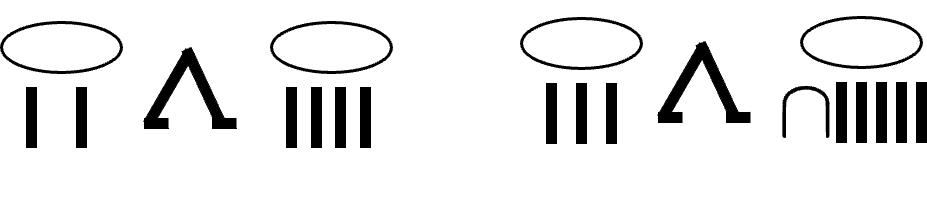
\includegraphics[scale=0.3]{img/sum-egyptian-fractions}
 \caption{左:$\frac{1}{2} + \frac{1}{4}$ \qquad 右:$\frac{1}{3} + \frac{1}{15}$}
 \label{fig:sum-egyptian-fractions}
\end{figure}

迄今为止,没有发现直接的文献,揭示为何古埃及人将分数系统设计为不同的单位分数之和。我们只能加以猜测。有一则传说故事说:老父亲在临终前希望把自己的遗产分给三个儿子。给大儿子$\frac{1}{2}$,二儿子$\frac{1}{3}$,小儿子$\frac{1}{9}$。但全部遗产只是17匹马。三个儿子不知道如何分配,也不愿杀死马进行分割。他们于是去请教村里的长者。老人将自己的一匹马借给了他们。于是大儿子分得$18 \times \frac{1}{2} = 9$匹马,二儿子分得$18 \times \frac{1}{3} = 6$匹马,小儿子分得$18 \times \frac{1}{9} = 2$匹马,剩余$18 - 9 - 6 - 2 = 1$匹马,恰好就是智慧的老人借给他们的那一匹。于是物归原主,老人牵走了他自己的马。这个传说故事用埃及分数解释就是

\[
\frac{17}{18} = \frac{1}{2} + \frac{1}{3} + \frac{1}{9}
\]

尽管脍炙人口,这个传说\underdot{不可能}是古埃及人发展分数系统的初衷。我们在各个民族,包括阿拉伯、印度、犹太、中国的民间故事中都发现了类似的故事。分配的遗产有马、骆驼、大象等动物,数量也有不同。例如三个儿子按照$\frac{1}{2}$、$\frac{1}{4}$、$\frac{1}{6}$分配11个动物,体现为:

\[
\frac{11}{12} = \frac{1}{2} + \frac{1}{4} + \frac{1}{6}
\]

\cref{qn:three-sons}给出了所有能这样进行分配的数量和比例。我们最早在十八世纪伊朗哲学家纳拉奇(Mulla Muhammad Mahdi Naraqi)的著作中看到此故事的文字记载。

读者朋友们,你觉得古埃及人为何如此设计他们的分数系统呢?

\section{古巴比伦的分数}

\section{古代中国的分数}
\label{sec:chinese-fractions}

\section{印度分数}

\section{小数}

\section{分数的其它形式}

\section{数系的扩展}

\begin{Exercise}[label={ex:fractions}]
\Question{找出三个儿子按照$\frac{1}{a}$、$\frac{1}{b}$、$\frac{1}{c}$分配$n$个动物的所有可能数值和比例。要求大儿子分得的财产多于二儿子,二儿子分得的财产多于小儿子。\label{qn:three-sons}}
\Question{如果你会编程,请用计算机枚举上面的所有解。}
\end{Exercise}

\begin{Answer}[ref={ex:fractions}]
\Question{找出三个儿子按照$\frac{1}{a}$、$\frac{1}{b}$、$\frac{1}{c}$分配$n$个动物的所有可能数值和比例。要求大儿子分得的财产多于二儿子,二儿子分得的财产多于小儿子。}
\Question{如果你会编程,请用计算机枚举上面的所有解。}
\end{Answer}

\ifx\wholebook\relax \else
\section{参考答案}
\shipoutAnswer

\begin{thebibliography}{99}
%% \subimport{inc/}{bib-zh-cn}
\end{thebibliography}

\expandafter\enddocument
\fi
